
\chapter{Abstraction, Act 2}

\section{Where we're going}

So far we've dealt mostly with modeling populations, and we have done
so using discrete time models -- models where we assume, either for
simplicity or for structural reasons, that it makes sense to talk
about the state of the system at discrete points in time.

To do this, we've utilized a couple of pieces of formalism: stock and
flow diagrams, which qualitatively represent our understanding of what
quantities we are tracking, and how they evolve in time, and
difference equations, which more quantitatively express the model.

We've also worked on implementing models, using both MATLAB and using
some analytical tools (e.g., finding equilibria for a set of
difference equations). We've started to validate models -- mostly
using comparison to data and common sense -- and we've begun to go
beyond using a model to generate a time series.

We're now going to iterate again on the modeling process.  You'll see
some new stuff along the way:

\begin{itemize}
\item We will begin dealing with continuous time models -- models in which we assume that the system is evolving constantly in time, and in which we are able, in principle, to ask about what the state of the system is at any given time.
\item We'll begin looking at systems other than populations -- initially, thermal systems, and shortly after that, physiological systems.
\item We'll be seeing some new mathematical formalism -- differential equations
\item We'll be learning some new implementation approaches for differential equations -- both analytical and numerical
\item We'll be introducing some new validation ideas, such as limiting behavior
\item We'll be starting to think about how to be more sophisticated in doing work with models, both by introducing lumped parameters, and by thinking about figures of merit.
\item Most importantly, we'll be studying systems that behave according to the law of physics.  To determine the behavior of a function in your model, you will now be able to rely on existing validated physical models (such as models for solar radiation and heat loss through walls). 
\end{itemize}

At the same time, our old friend the stock and flow is still with us, and we'll resurrect difference equations to help us make sense of differential equations -- so the territory is not really all that new...

\section{Differential Equations and Stocks and Flows}

In modeling populations, we used difference equations.  For example, we modeled the elephant population in year $n+1$, $E_{n+1}$, as depending on the population in year $n$:
$$E_{n+1} = E_n + bE_n - d E_n$$
As we move into modeling thermal and other systems, we are going to begin using a different type of mathematical formalism:  the {\it differential equation}.

At its core, a differential equation is simply an equation that involves derivatives.  A very simple example would be
$$\frac{df}{dt} = 0$$
which states that the function $f$ has a derivative of zero.

While we're going to develop more sophistication with differential equations as we go along, for now you can think about a differential equation as something that states how a rate of change (a``differentia'') in one variable is related to other variables or itself.  For example, 
$$\frac{dx}{dt} = C(x_0-x)$$
says that the rate of change of  $x$ with respect to $t$ is proportional to how far $x$ is from $x_0$.  If $x<x_0$, then the rate of change of $x$ is positive, and if $x>x_0$, the rate of change is negative.  

Differential equations tie very directly to stocks and flows:  a flow is something that causes a stock to change, so the total rate of change of a given stock should depend on what flows are attached to it.  In general, if you are translating a stock and flow to a differential equation (or vice-versa), 
{\bf each stock should have a differential equation associated with it, and that equation should have the same number of contributions as there are flows into and out of the stock.}   

\subsection{An Example: The Bathtub Problem}

Let's try a simple example that lets us connect a simple physical situation to a stock and flow, which we cn then use, in turn, to develop a differential equation.

Imagine a tub full of water. No water is entering the tub but some water is flowing out a drain in the bottom of the tub, as shown below:

\beforefig
\centerline{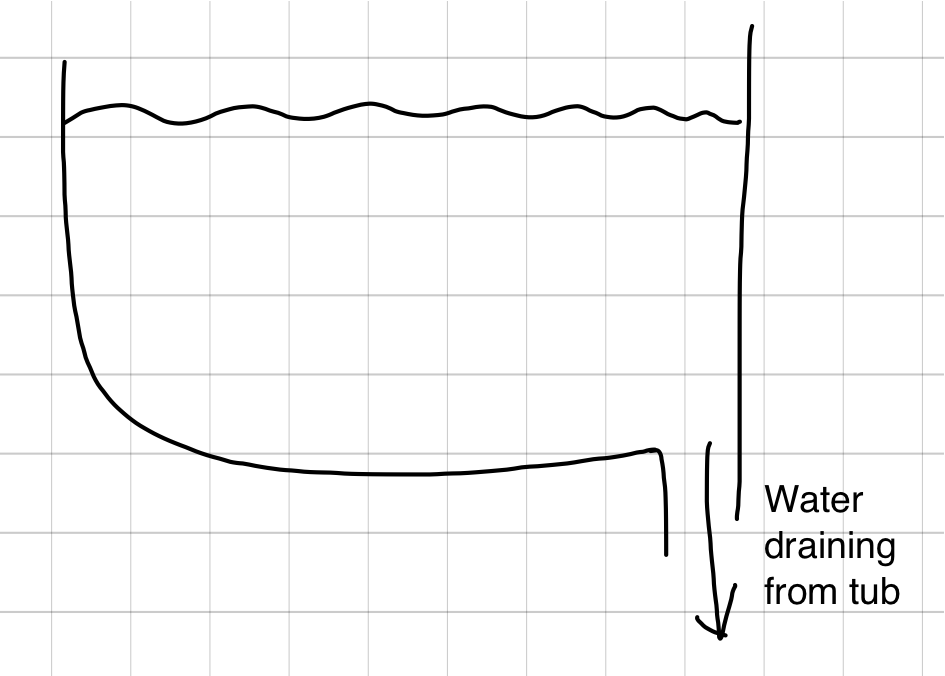
\includegraphics[height=1in]{figs/Tub1Schematic.png}}
\afterfig

We would like to track the rate of change of water in the tub over time. Let's start with a stock and flow diagram.

\beforefig
\centerline{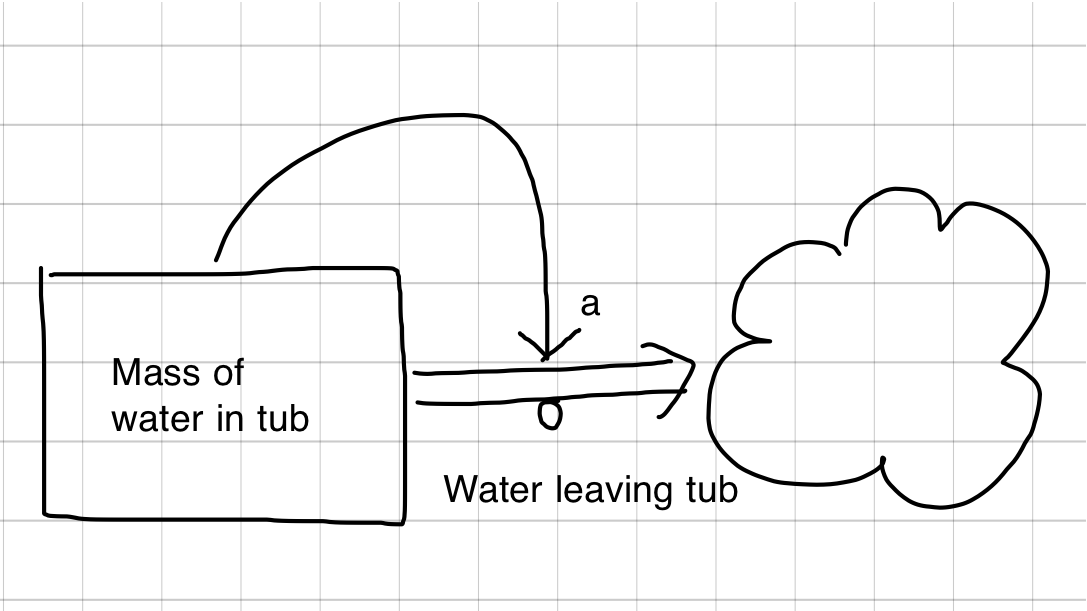
\includegraphics[height=1in]{figs/Tub1StockandFlow.png}}
\afterfig

Note that we've chosen the {\it mass} of water in the bathtub to keep track of. We could have kept track of the volume of water as well, but for now, mass it is.  The stock and flow diagram shows one stock (the mass of water in the tub) and one flow (the rate of water leaving through the drain). The rate of water leaving through the drain is dependent on the amount of water in the tub. \sidenote{You might think about this for a minute to make sure it makes sense to you intuitively. It has something to do with hydrostatics. You might see http://www.youtube.com/watch?v=2tBWfqKA0Tk for a physical example.} A physical law called the Bernoulli equation provides the details of this relationship, but for now, let's just say that the flow out is proportional to some constant, $a$, and the mass of water in the tub. 

If we wanted to write a difference equation from this stock and flow diagram, it would look like:

$$ m(t+1)=m(t)-am(t)$$

This simply says that the mass of water in the tub at time $t+1$ is equal to the mass of water at time $t$ minus the amount of water exiting the tub during that time step. If we were to continue our analysis using the difference equation, what time step would we choose? We could look at the state of things every 10 seconds, but this makes a lot more sense when we are dealing with a discrete stock that we can stop and count (i.e. 7 wolves, 100 primary schoolchildren, 800 sharks). Because our flows are not discrete chunks of stock (i.e. 4 moose/year), it makes more sense to use a continuous model. This is where differential equations come in. We can solve a differential equation so that we could look at the water in the tub at any time, not just every 10 seconds. But we're getting ahead of ourselves... let's write the differential equation and see what it tells us:

$$ \frac{dm}{dt}=-am(t)$$\sidenote{It may help to remember that $\frac{dm}{dt}\approx \frac{m(t+1)-m(t)}{\Delta t}$}

The differential equation tells us that the rate of change of mass in the tub per unit time is equal to the rate of water leaving the tub.
What if we made things more complicated, and turned on the spigot so that water is added at a constant rate, $c$ [kg/s], to the tub? Well, we could just modify our stock and flow diagram,

\beforefig
% Add second stock and flow figure here.
\centerline{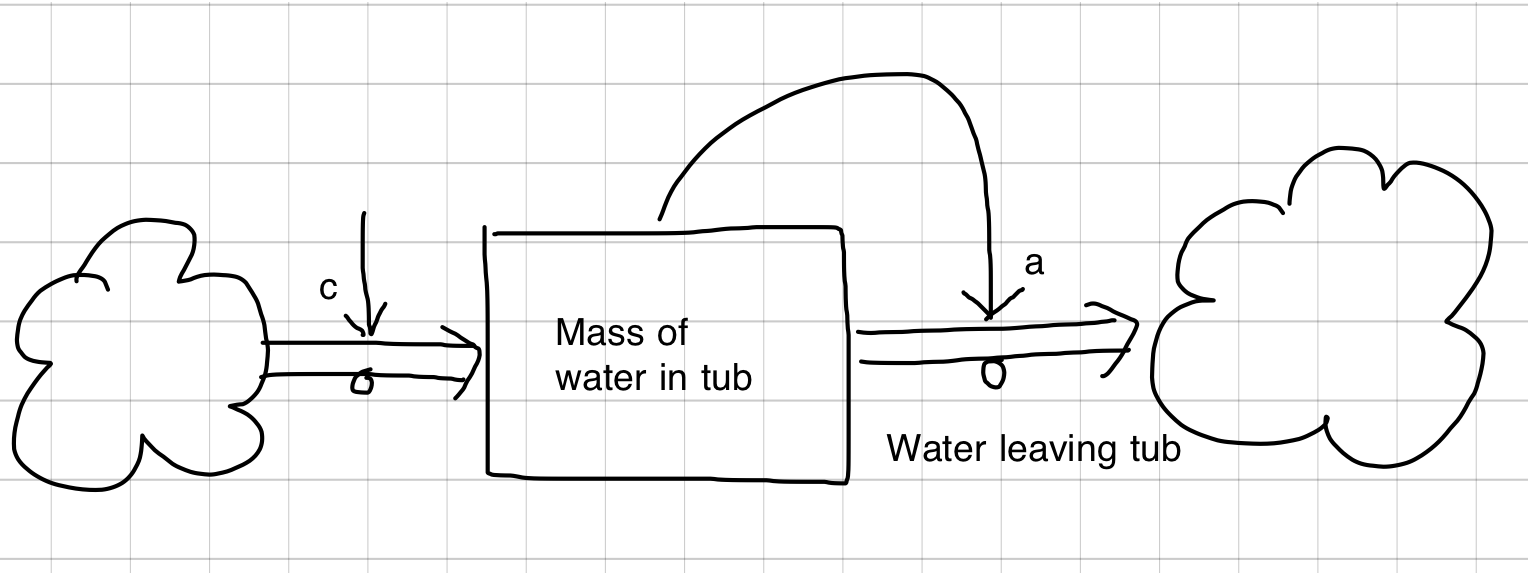
\includegraphics[height=1in]{figs/Tub2StockandFlow.png}}
\afterfig

and add the extra term to our differential equation:

$$\frac{dm}{dt} = c-am(t)$$

Finally, if we wanted to create a system with two stocks, we could add another tub of water emptying into our original tub, as follows:

\beforefig
% Add second stock and flow figure here.
\centerline{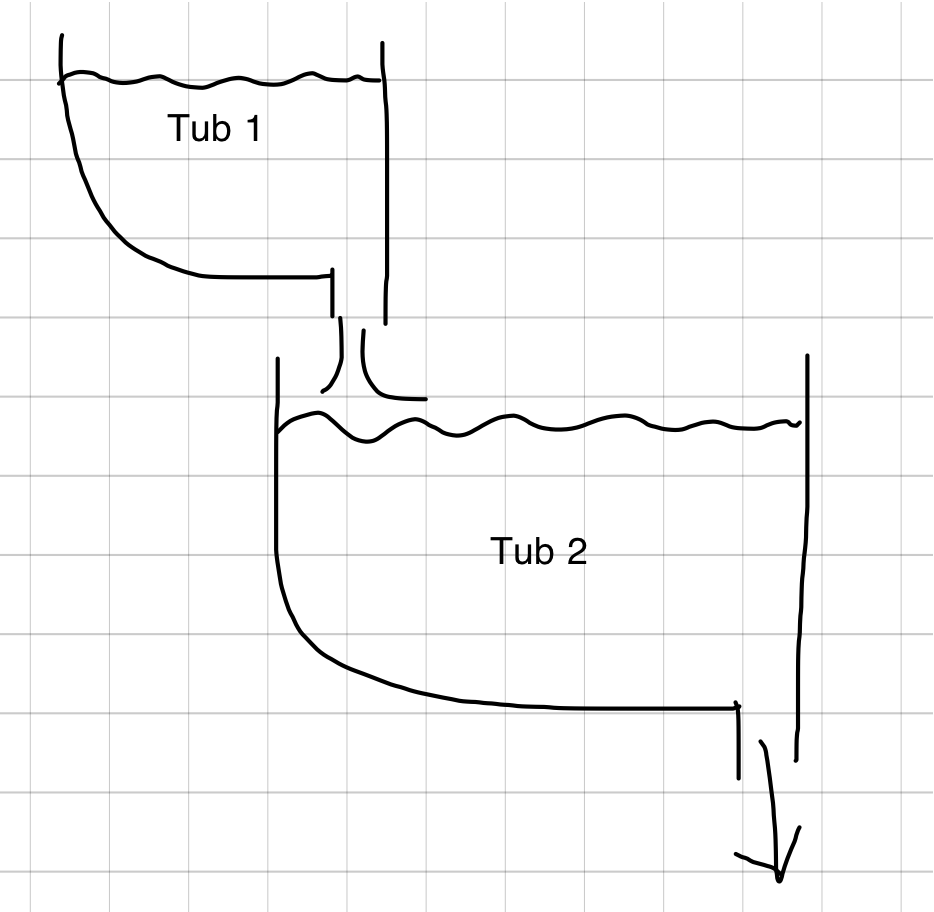
\includegraphics[height=1.5in]{figs/Tub2Schematic.png}}
\afterfig

\beforefig
% Add second stock and flow figure here.
\centerline{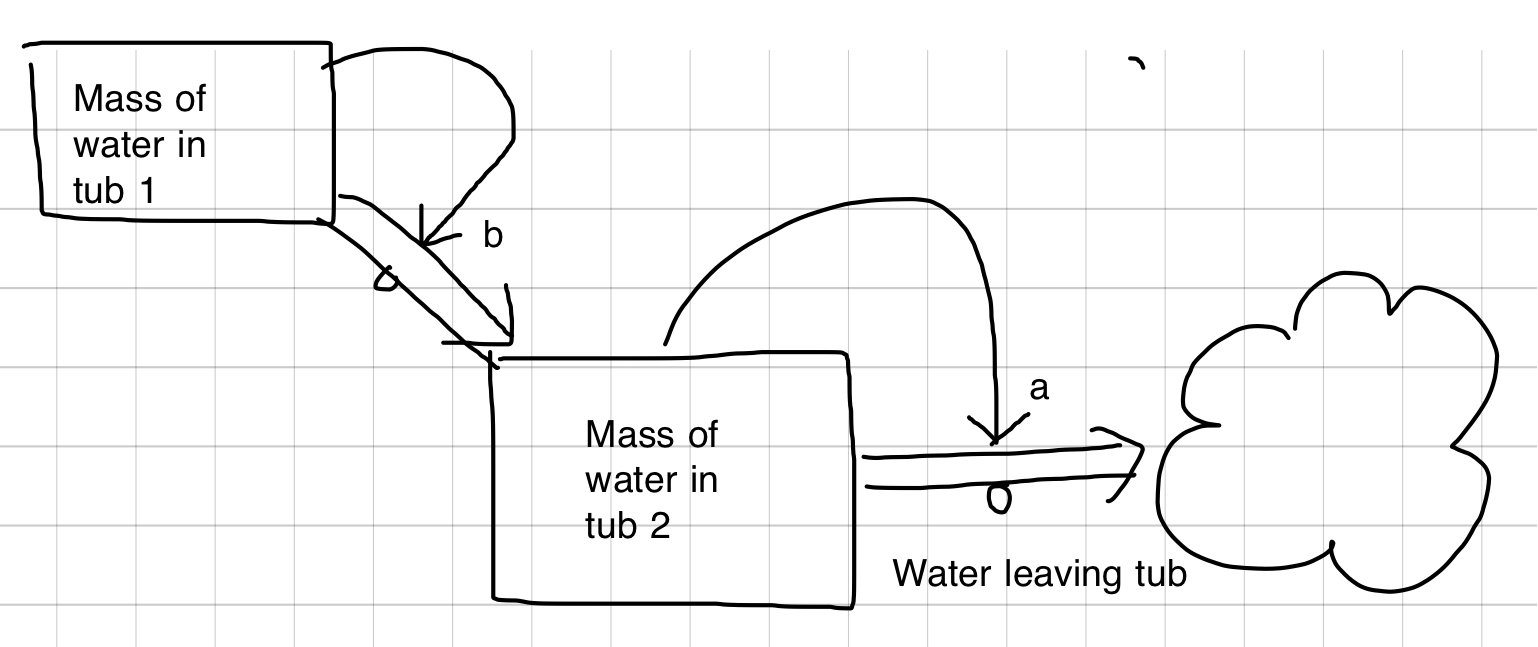
\includegraphics[height=1.5in]{figs/Tub3StockandFlow.png}}
\afterfig

and  write a system of differential equations (one for each stock):

$$\frac{dm_1}{dt} = -bm_1(t)$$
$$\frac{dm_2}{dt} = bm_1(t)-am_2(t)$$

 
 \section{Let's stop and take stock} 
 
In ModSim, we've been using stock and flow diagrams, as well as difference equations, and (starting now) differential equations.  In this section we ask two questions: (1) What do these different representations buy you? and (2) How do they relate to each other?

\begin{center}
\begin{tabular}{ | p{2cm} | p{5.5cm} | p{2.5cm}   | p{2.5cm}  |}
\hline
Type of representation & Bathtub Example & Advantages & Disadvantages \\
\hline
Stock and Flow & \vspace{0.05in} 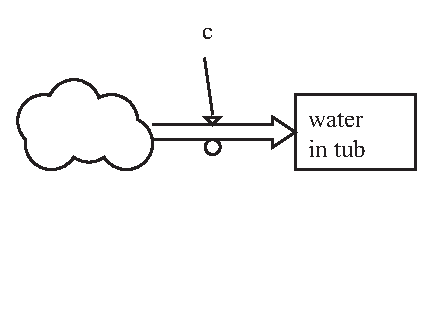
\includegraphics[height=.7in]{figs/stockandflowbathtub}\vspace{0.05in} & Easy to connect to physical system; conservation is explicit; very qualitative & Very qualitative \\
\hline
Difference equation & $$m(t+1) = m(t) + c$$ & Easy to implement. High level of formality.  Rigorous. & inappropriate for continuous systems, somewhat more difficult to interpret \\
\hline
Differential equation & $$\frac{dm}{dt} = c$$ & appropriate for continuous systems. High level of formality.  Rigorous. & inappropriate for discrete-time systems, somewhat more difficult to interpret \\
\hline
\end{tabular}
\end{center}



 \section{Example: Thermal Systems}

While it is tempting to think about thermodynamics as being all about temperature, it is really a very general science that is concerned with the question of how a system changes state as a result of various processes (heat flows, work, etc.).  

That idea -- that a system changes state as a result of processes -- should sound familiar, because it's the way we've been talking about stocks and flows.  Stocks represent the state of the system (e.g., how many elephants there are), and flows represent the processes by which the system changes (e.g., hunting).  

\subsection{State Variables}

in thermodynamics, we tend to be concerned with two different types of stocks:

\begin{itemize}
\item {\it Internal Energy} is perhaps the stock we'll encounter most frequently.  Internal energy is a measurement of the total energy contained in the system, both in the form of potential energy {\it within} the system (e.g., a compressed spring), and in the form of kinetic energy within the system (e.g., molecules moving around or vibrating).  Internal energy is denoted with a $U$, and (in SI units) has units of Joules.

\item {\it Mass} of a system can change as well, if the system has open boundaries -- i.e., if matter is allowed to go across the boundary.  Mass if typically denoted $m$, and has units of kilograms.

\item{\it Volume}, denoted $V$, can be thought of as a stock, although this requires a bit more brain stretching than mass or internal energy.  The units are, of course, meters$^3$.

\end{itemize}

The internal energy, mass and volume are all {\it extensive} variables, meaning that they are dependent on the {\it extent}\sidenote {This is an excellent mnemonic for remembering the difference between extensive and intensive variables.} (or size) of the system.  If you decide to analyze a system that is twice as big, the mass will be higher, the volume will be higher, and the internal energy will be higher. 

Contrast this with and {\it intensive} variable, which does not depend on the size of this system. This is perfect time to discuss temperature, and to highlight that {\bf temperature is not a stock}. This is because temperature is an {\it intensive} state variable, which means that it does not depend on the size of the system. Doubling the size of the system does not increase the temperature of the system, and it does not make sense to think about temperature ``flowing''. Of course, the fact that temperature is neither a stock nor a flow doesn't mean it's not important.  Intensive state variables you are likely to encounter in thermal systems include:

\begin{itemize}
\item {\it Temperature}, denoted $T$, has units of Kelvins.
\item {\it Pressure}, denoted $P$, has units of Newtons/meter$^2$.
\item {\it Density}, denoted $\rho$, has units of kg/meter$^3$.
\end{itemize}

\subsection{Processes for Changing Internal Energy: Heat and Work}

The internal energy of a system can change due to heat being added to the system: put a pan on the stove, and when you turn on the flame, you will begin increasing the internal energy of the pan.   Internal energy can also be changed by doing work on the system, or by having the system do work on something else.  For example, in a car engine, expanding gas pushes up the pistons in the cylinders; this work done by the gas reduces the internal energy of the gas.  In general,
$$\Delta U = Q - W$$
where  $\Delta U$ is the change in the internal energy of the system, $Q$ is the heat that is added, and $W$ is the work done {\it by the system} \sidenote{The typical sign convention for heat transfer is positive for heat transfer into the system, and negative for heat transfer out the system. Work typically has the opposite sign convention, hence the negative sign in the equation. Ask Jessica for an easy way to remember this.}  Note that both heat and work have units of energy here.  

Heat is (rather circularly) defined as energy that is transferred by means other than doing work; examples of heat flow mechanisms include conduction (if you touch something hot, energy flows into you from the hotter object), radiation (e.g., energy radiating onto your skin from the sun as you lie on the beach), convection (energy lost to a surrounding fluid like air or water) and mass transfer (e.g., energy being carried away in evaporating water).  Unfortunately this definition of heat tends to be at odds with our typical usage of the word -- when we talk about ``turning up the heat'', we typically mean that we wish to increase the {\it rate} of heat transfer. Thus, we often use the word ``heat'' to refer to a flow, which, while just fine in casual usage, is very wrong indeed in the world of physics and engineering...

Work includes both traditional mechanical work (i.e., exerting a force through a distance -- as in moving a piston) and other forms of work (e.g., charging a battery).

\subsection{Two Simple Examples}

Let's think through two simple examples to illustrate the stock and flow picture of thermodynamics.

{\it Example 1: Loaf of Bread.} Imagine that I have made you a loaf of bread. I take it out of the oven, place it on a wire mesh cooling rack on the counter, and tell you that you cannot eat it until it reaches room temperature. You now are interested in knowing how long that will take.

First, you would abstract the situation by saying, ``It's a loaf of bread in thermal contact with the air on all sides (ignoring the wire mesh cooling rack to keep it simple).'' In this case the ``system'' is the loaf of bread and the ``surroundings'' are everything else. 

\beforefig
\centerline{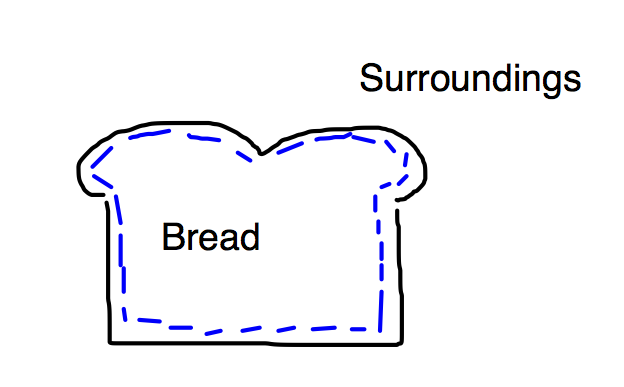
\includegraphics[height=1in]{figs/bread.png}}
\afterfig

Now, think about the stocks you might keep track of here. First, we know that mass can be a stock, but it turns out that not much is changing with the mass as the bread cools. We could also keep track of the volume of the bread, but that is also not changing with time. However, it is likely that the size (and therefore the volume) is important. How quickly the loaf will cool definitely has something to do with the size of the bread -- a teeny tiny loaf would likely cool faster. So the size or volume is something we'll make sure to include as an important parameter.

A second stock that makes sense to keep track of is the internal energy. We haven't talked about this yet (keep reading!), but the internal energy of a material is often directly related to the temperature of the material, so by keeping track of internal energy, we can likely predict the time at which we will reach some temperature.

We've identified one important parameter (the volume), a stock we will keep track of (the internal energy) and now we want to identify the flows. How will the internal energy of the bread change? It will decrease as heat is lost to the air around it. So we've identified the one flow in this example.

\beforefig
\centerline{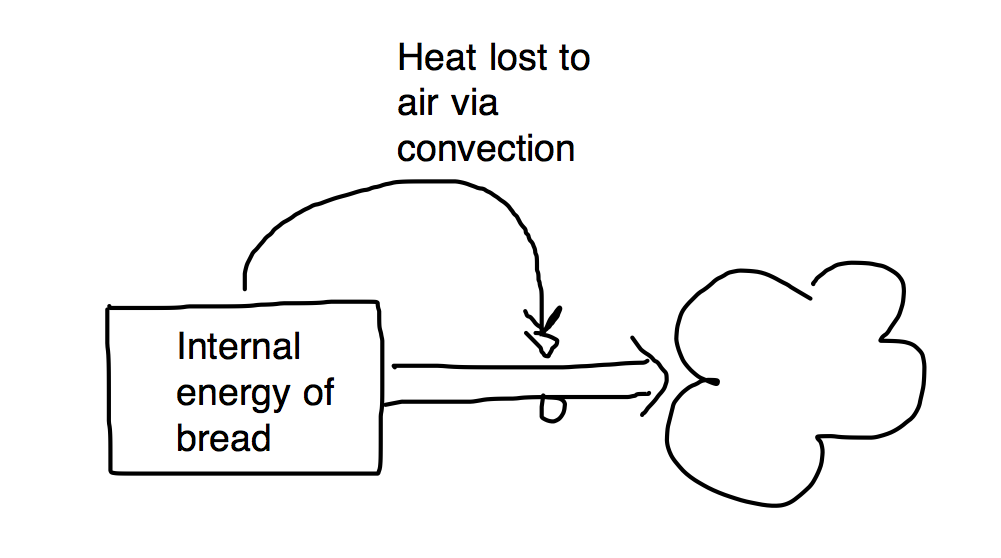
\includegraphics[height=1.7in]{figs/breadstockandflow.png}}
\afterfig

The next step would be to identify the relationship between the size of the bread and the heat lost to the air, but we'll look at one more example of abstracting a thermal system before we dive into the details (see the section on Convection if you'd like to skip to the details).

{\it Example 2: Pot of Water.} Imagine we have a pot of water on a stove, and we're interested in knowing what will happen to it in the future.  In abstracting this, you might choose to say ``It's a mass of water, in thermal contact with a pan.  The bottom of the pan is in thermal contact with a burner, and the sides of the pan are surrounded by air.''  Let's say that we are really interested in what happens to the {\em water}, so we'll say that the ``system''  is the water in the pan, and the ``surroundings'' are everything else (pan, air, burner).  (Of course, you could make a different choice here -- e.g., you could decide that the system included the pan.)  

\beforefig
 \centerline{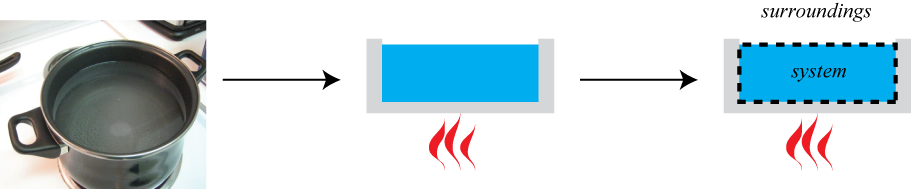
\includegraphics[height=1in]{figs/ThermalSystemAbstraction.png}}
\afterfig

Once you've decided what your system is, decide what stocks make sense to keep track of. Unlike the loaf of bread there is a distinct possibility that some mass may leave the system by evaporating (assuming your pan is not covered, and the temperature of the water is allowed to reach the boiling point). So we'll consider mass to be a stock, and the rate of water leaving by evaporation to be a flow. 

In order to know whether we do reach the boiling point temperature, it is again useful to keep track of how the internal energy of the water changes (again, as you will find out oh so very soon, the internal energy is a function of temperature). How will the internal energy of the water change? It will increase as heat is transferred from the burner, to the pan, and finally to the water. It will decrease as heat is lost to the pan and then to the surrounding air. Finally, as the mass of the system decreases due to evaporation, the internal energy will also decrease -- there will be less water in the system to actually have internal energy.\sidenote{This is what is known as an {\it open} system; where mass can cross the system boundary. In a {\it closed} system, mass cannot cross the system boundary, but heat can.}  So, a simple stock and flow might look like this:

\beforefig
 \centerline{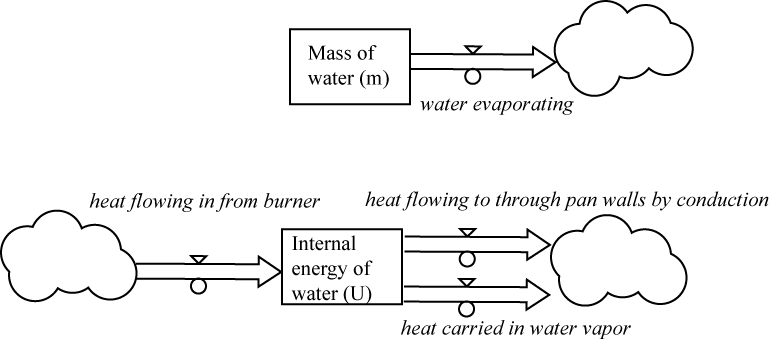
\includegraphics[height=2in]{figs/WaterInPanSimple}}
\afterfig

Of course, we've not yet defined anything about how these processes work or how to model them: the flows in this stock and flow diagram are only defined in the most hand-wavy way.  But we at least have a general picture of what is going on, and now can begin thinking about models for temperature and heat flow.

\section{Thermodynamic Relationships}

In order to model the flows in a thermodynamic system, we need to deal with a couple of issues:  first, {\it how does temperature relate to internal energy?}, and second, {\it what are the mechanisms for heat flow?}.  We deal with these two questions in the following sections.


\subsection{Internal Energy, Temperature and Specific Heat}

Although it might make perfectly good sense to talk about the amount of internal energy in a system, the reality is that this is not a quantity that we measure directly -- rather, we tend to measure temperature.  

Temperature, it turns out, is closely related to the internal energy of a system. What do you think would happen to the internal energy of a mass of water if heat were added to it? How do you think the temperature would change? Let's do the thought experiment and assume our water starts at room temperature (about 20 C or 293 K) and is heated to just below the boiling point (99 C or 372 K). The temperature in increasing (because we are adding heat) and the internal energy is also increasing. Here's what a plot of internal energy, $U$ versus temperature, $T$ might look like. 

\beforefig
 \centerline{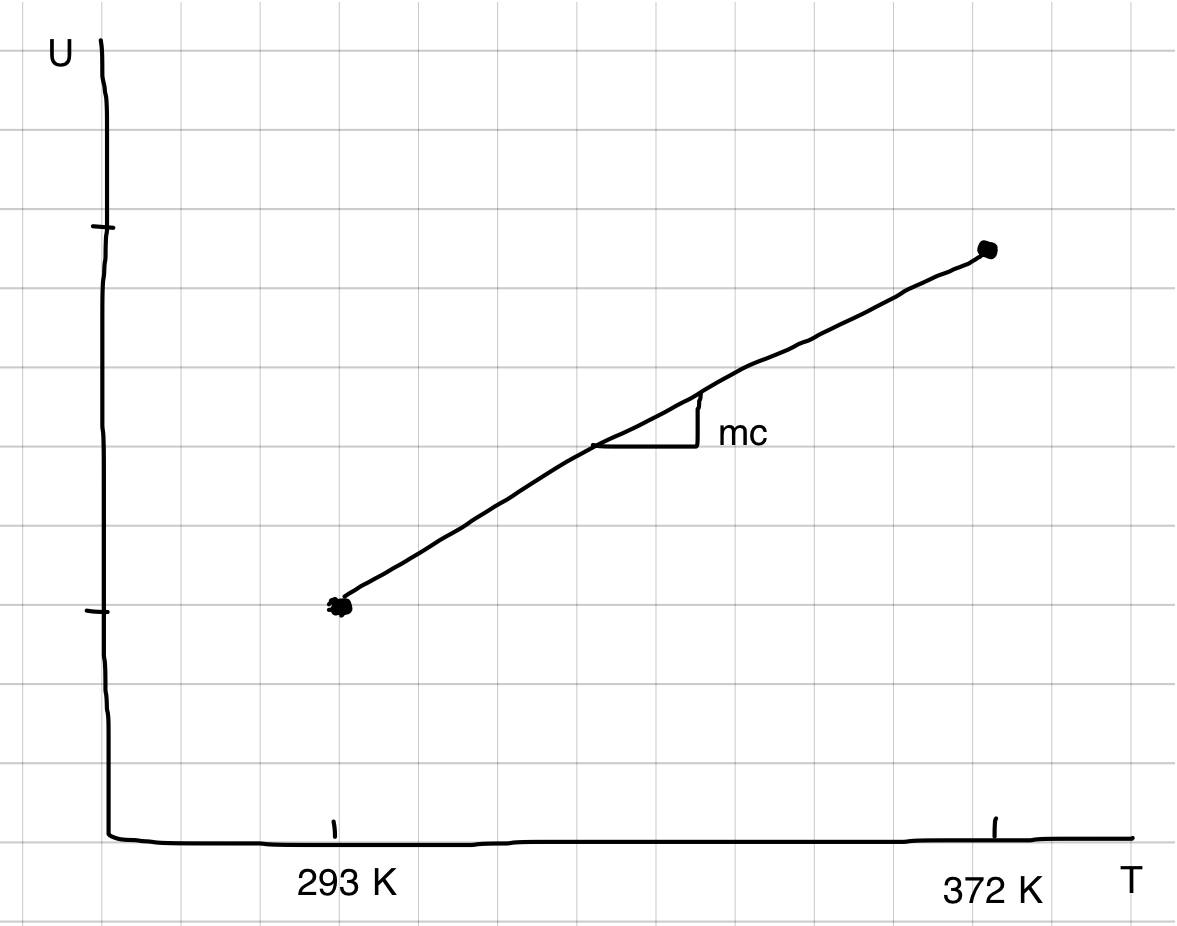
\includegraphics[height=3in]{figs/SensibleHeatFigure.png}}
\afterfig

Note the slope of the line: the change in the internal energy is {\it nominally} (this is a model, after all) linearly proportional to the change in temperature:

$$ \Delta U = m c \Delta T$$

where $m$  is the mass of the system, $c$ is the {\it specific heat} (units of J/K-kg), and $\Delta T$ is the change in temperature.

You've probably heard of specific heat before; it's the amount of heat needed (in Joules) to raise 1 kg of mass by 1 degree Kelvin. Note that specific heat, $c$, is an intensive property. It is defined per unit mass (kg is in the denominator) and therefore is relevant for any size system. It's a property of a material and is not a function of mass or volume.

Another property can be defined by combining the mass of a system and its specific heat.

$$C = mc = \frac{\Delta U}{\Delta T}$$ 

This is known as the {\it heat capacity} or the {\it thermal mass} of a system, and simply tells you the amount of energy needed to raise the temperature 1 degree. Heat capacity is an extensive property.

In thermodynamics, we often think about properties of a system both microscopically and macroscopically. Microscopically (or in the field of statistical mechanics), one way to define temperature is to relate it to the average kinetic energy of a particle in the system.  For example, in a monatomic gas, the average kinetic energy of an atom in the gas is given by
$$<KE> = \frac{3}{2} k_B T$$
where $k_B$ is the Boltzmann constant, a fundamental physical constant with the value of $1.380 \times 10^{-23}$ m$^2$ kg s$^{-2}$ K$^{-1}$

The internal energy is a functionf of the kinetic energy of the particles, which is a function of temperature, which allows us to finally state (although our thought experiment has already shown thist ), that:

$$\Delta U \propto \Delta T$$


\section{Mechanisms for Heat Transfer}

\subsection{Just tell me the power}

In some situations, heat transfer can be thought of simply as a constant power process.  For example, if you put a 500 W immersion heater into a cup of water, it's a pretty good model to simply assume that the 500 W heater is delivering 500 W to the water.  Thus the rate of change of the internal energy would be

$$\frac{dU}{dt} = 500 W$$

Your metabolism acts a bit like an immersion heater -- the basal metabolism rate is around 60 W.

\subsection{Conduction}

{\it Conduction} is a heat transfer mechanism that involves heat flow through matter, due to differences in temperature between one point and another.  In conduction, the physical mechanism (on a microscopic scale) for heat transfer is vibration of particles, as opposed to bulk motion of particles. For example, if you hold a metal rod, and stick one end into a campfire, the atoms in the rod at that end absorb energy from the fire, and start to vibrate more.  These vibrating atoms knock into their neighbors, causing them to vibrate, and so forth.  Thus, the end that you are holding will eventually get hot as energy is carried down the rod by these vibrations: heat flows from the hot end to the cold end, which leads to the cold end getting warmer. 

One common physical system for which the heat conduction model comes in very handy is heat loss through a wall. Let's imagine you build a house of blue foam, with 4 inch thick blue foam walls. How much heat might be lost through a wall? What if the internal and external walls were at the same temperature? Well, the Second Law of Thermodynamics (and your intuition, I hope) tell us that heat flows from hot to cold, so if there is no temperature difference, no heat will flow. What if the internal wall is just a little hotter than the external wall? One might venture to guess that a little bit of heat will flow. What if the internal wall were much hotter than the external wall? A lot of heat will flow. You get the picture.

\beforefig
\centerline{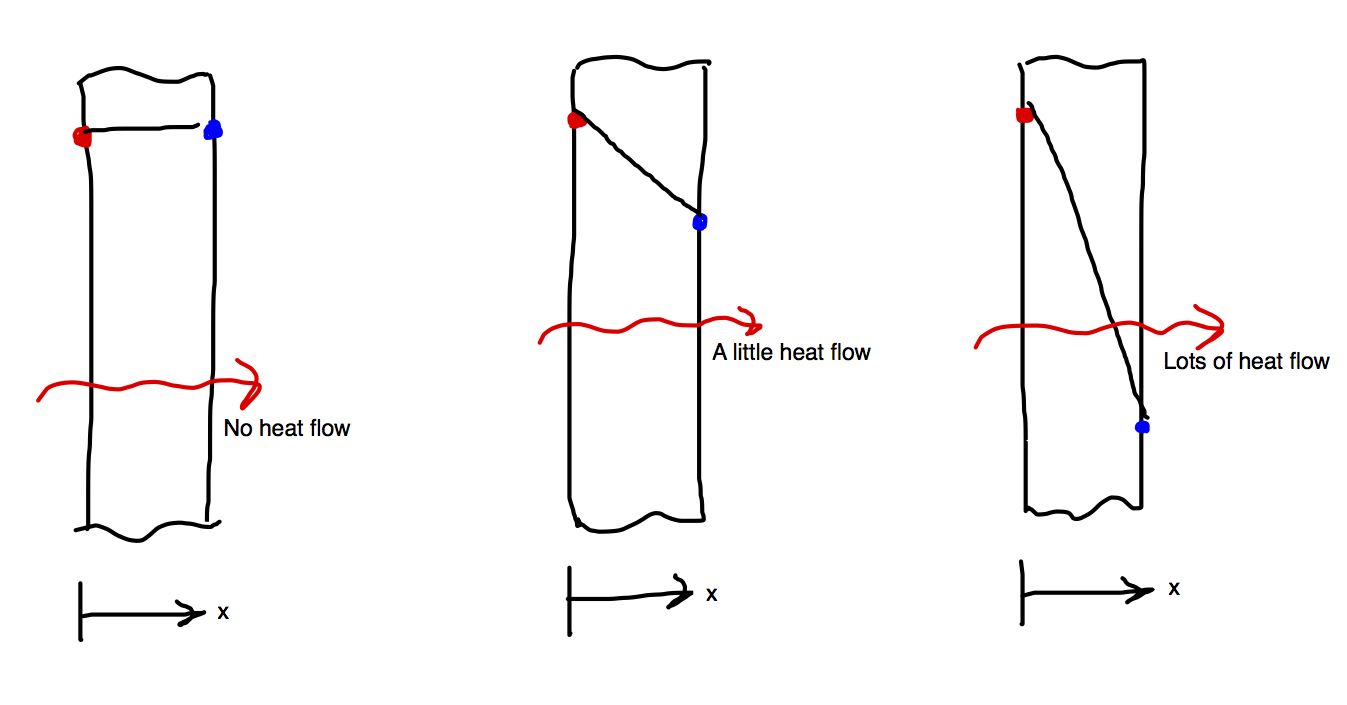
\includegraphics[height=2in]{figs/wallheatflow.png}}
\afterfig

However, what if I was trying to save money and gave you 2 inch thick blue foam to use instead? You might expect that you would lose {\it more} heat through the thinner wall. What if I gave you 4 inch thick concrete instead of blue foam? Now, this could get interesting. It would depend on how well concrete conducts heat as compared to blue foam. This is typically captured in another material property called the {\it thermal conductivity}, $k$ (units of W/m-K)\sidenote{The units of thermal conductivity have a``per unit time'' built in since 1 Watt = 1 Joule/s. Hence, thermal conductivity relates a temperature difference to a {\it rate} of heat transfer.} Finally, you might expect that you would lose more heat through a larger wall (higher area) than a smaller wall. 

All of these factors are captured in Fourier's law (which is, of course, a very good model, not a law), which tells us that the rate of heat flow $\dot{Q}$ is proportional to the temperature difference, the thermal conductivity $k$ and the area $A$, and inversely proportional to the thickness of the wall $d$.

$$\dot{Q} = -\frac{kA}{d} \Delta T $$

The whole proportionality constant relating temperature difference to heat transferred, $\frac{kA}{d}$ is sometimes known as the thermal conductance, $K$, which is a measure of how easily the heat can be transfered through the body (and is an extensive property). You might expect a wall with a larger surface area to have a higher thermal conductance (i.e., bigger houses lose more heat through the walls than smaller houses).  Furthermore, the thicker the wall, the less heat I expect to travel through the wall, and the lower the thermal conductance.

There is one other interesting thing about Fourier's Law: the minus sign. Heat flows from hot to cold (left to right in the figures above, which is the positive x direction), but the temperature gradient is defined as $T(x+d) - T(x) $ which would be negative in the examples above. Hence the minus sign in Fourier's Law to indicate the direction of heat flow is opposite from the temperature gradient.

{\it Conduction Example.}  You pour hot coffee into a ceramic mug with a lid and let it sit on the counter.\sidenote{Maybe a nice little red mug like this -- 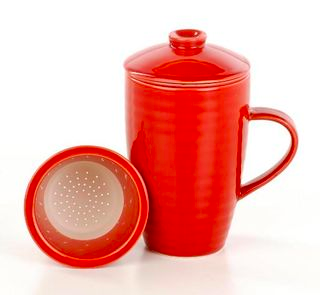
\includegraphics[height=2in]{figs/mugwithlid.png}}  You wonder how long it might take to cool to a drinkable temperature. The coffee starts at a temperature of 370 K,\sidenote{From Wikipedia: "The Kelvin scale is an absolute, thermodynamic temperature scale using as its null point absolute zero, the temperature at which all thermal motion ceases in the classical description of thermodynamics." Also, 0 C = 273.15 K and 100 C = 373.15 K.} $T_{init}$  and the surrounding room is 290 K, $T_{env}$. Our goal is to find out how the internal energy of the coffee changes over time, and to use Fourier's Law of Conduction to help us determine that.

We'll start by thinking about how to abstract this.  We'll define our system as the coffee, and the only stock we care about is the internal energy of the coffee (since no mass will enter or leave the system -- the lid on the mug will prevent evaporation).  The flow of energy into the coffee from the environment will be governed by a few things:  the environmental temperature, the temperature of the coffee (which, in turn, depends on the internal energy of the coffee), and the conductance of the ceramic mug's walls.  So, qualitatively, we might represent the model like this:

\beforefig
\centerline{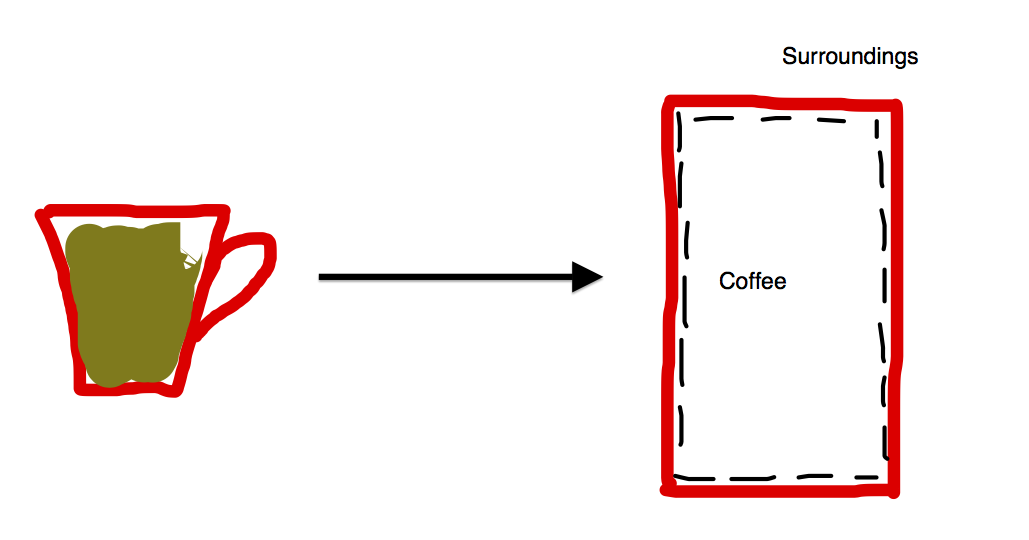
\includegraphics[height=1in]{figs/coffeeabstraction.png}}
\centerline{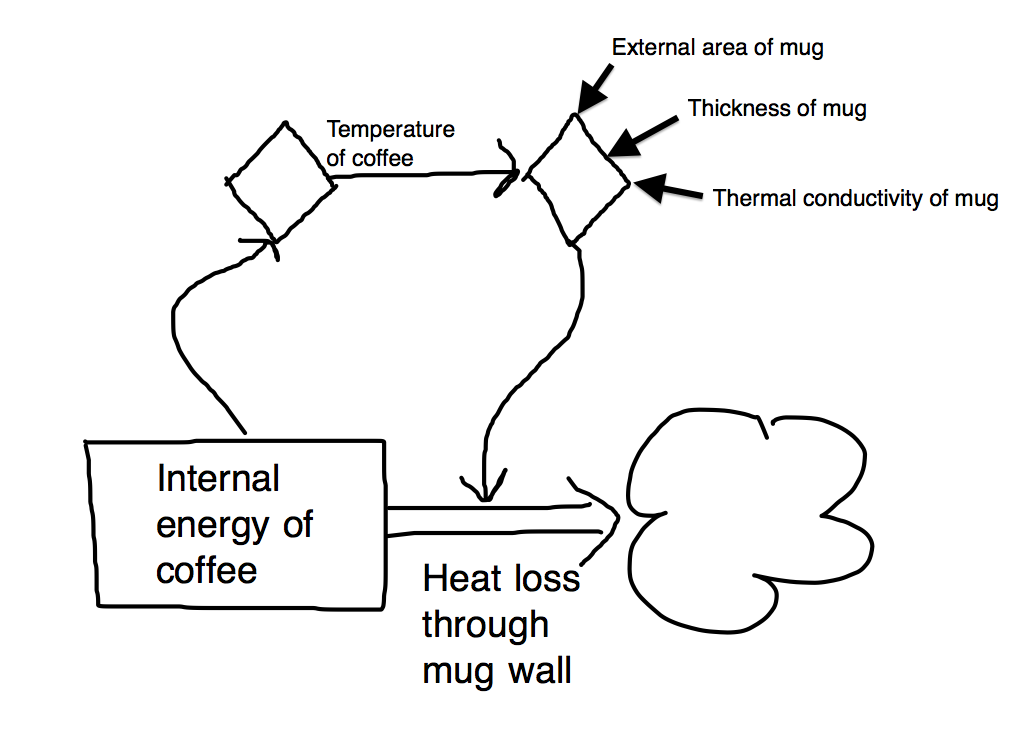
\includegraphics[height=2in]{figs/coffeestockandflow.png}}
\afterfig

Now, if we want to get quantitative about this, we'll need to somehow figure out (1) how to get the temperature from the internal energy (which involves re-reading the section above!), and (2) how to handle the heat loss due to conduction through the ceramic walls. Let's start with our general statement of how internal energy of a system can be changed:

$$\Delta U = Q - W$$

and on a per unit time basis:

$$\frac{d(\Delta U)}{dt} = \dot{Q} - \dot{W}$$

In this case there is no work being done on or by our system (the coffee is just sitting there!) so the only way the internal energy of the coffee will change is by heat transfer. We can use Fourier's Law to determine the rate of  heat transfer, $Q$:

$$\dot{Q} = \frac{kA}{d}\Delta T = K\Delta T$$

Thanks to the wonders of the world wide web, I find that the ceramic used in coffee mugs has a thermal conductivity, $k$, of 15 W/m-K.  Thus,

$$K = k A/d$$

where $A$ is the surface area (here, the area of the mug), and $d$ is the thickness of the mug walls.  Assuming my mug is 15 cm high and a 4 cm radius the area will be $2\pi \times 4 \times 15+2\pi \times 4^{2}=289 \textup{cm}^{2}=.0289\textup{m}^{2}$. We can estimate that the wall of the mug is about 0.7 cm thick. Then the thermal conductance is:

$$K = \frac {15 \times 0.289 }{0.007}=0.03$$

$\Delta T$ is $(T_{coffee} - T_{env})$, and we will assume that the inner temperature of the mug wall is the same as the current coffee temperature, and that the outer temperature of the mug wall is the same as the ambient temperature. To determine the current coffee temperature at a given point in time, we need to know how much heat has been lost to that point, which will tell us how much the coffee temperature has decreased. Using an equation from the previous section, we find that:

$$\Delta U_{coffee}=mc_{coffee}(T_{coffee}-T_{init})$$

and

$$T_{coffee}=T_{init} + \frac{\Delta U_{coffee}}{mc_{coffee}}$$

So, the rate of change of the internal energy will be given by
$$\frac{d\Delta U_{coffee}}{dt} = K (T_{env}-T_{coffee}) = 0.03\left(290 - \left(370+\frac{\Delta U_{coffee}}{mc_{coffee}} \right) \right)$$

Note that our final differential equation here does not explicitly contain the temperature of the coffee; rather it expresses the rate of change of internal energy in terms of the internal energy.

One of the confusing things about this model is the extent to which a body with a heat capacity can, in itself, be a thermal conductor.  For example, when you foolishly put one end of a metal rod in a campfire, the rod's internal energy increases, and at the same time there is heat flow within the rod.   Similarly, in a house, the walls of the house both conduct heat to the outdoors, and hold some amount of the house's internal energy.

One way to deal with this is to separate the object into one or more lumped thermal masses, connected by appropriate thermal conductance(s).  For example, we might choose to break the rod into two parts, or three parts, or four parts, or 1000 parts:

\beforefig
 \centerline{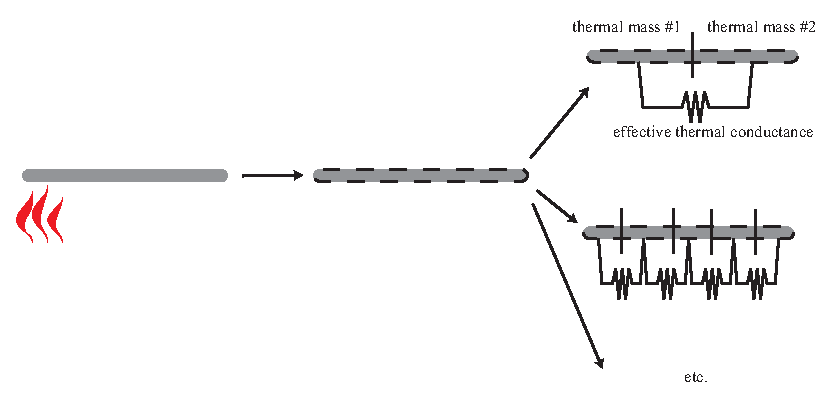
\includegraphics[height=2in]{figs/BreakingUpARod}}
\afterfig

Later (like next semester) we'll deal with this in more detail -- for now, the key idea is that you pull the stock apart from the flow:


\beforefig
 \centerline{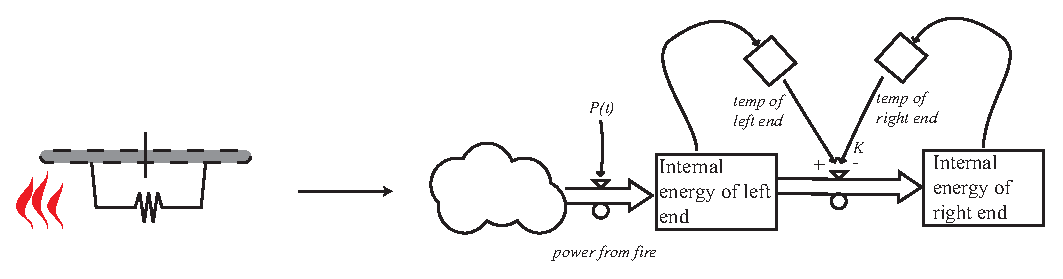
\includegraphics[height=1in]{figs/RodStockAndFlow}}
\afterfig

When you decide how to break things up, it's important to think about the {\it relative} conductance of different parts of the system.  For example, if half of your rod was made of gold (which has a very high thermal conductivity) and the other half was made of wood (with a low conductivity), you would likely NOT want to break the gold portion up -- heat will travel much faster in the gold than in the wood, so it's probably safe to guess that the temperature of the gold will be relatively uniform -- so breaking the gold up into little chunks might not be worth the effort. 

\subsection{R Values, U Values, K Values, and all that}
It is worth taking a moment to highlight some of the different ways that thermal conductivity, conductance, resistivity, and resistance are talked about.

Thermal {\it conductivity} is an intensive material property -- e.g., styrofoam, regardless of its shape, has a particular thermal conductivity -- and it tells you how well a particular type of material conducts heat.  Higher thermal conductivity implies that heat travels more easily in the material.  Thermal conductivity is denoted with a lower case $k$, and (in SI units) has units of W/K-m.  Typical values of $k$ range from about 0.04 W/K-m for fiberglass insulation to 400 W/K-m for copper.
Thermal {\it resistivity} is simply the inverse of thermal conductivity; usually you'll find conductivity listed, though.

Thermal {\it conductance} is a property of a given configuration of a particular material that connects one thermal mass to another.  It describes the rate of heat flow between the two bodies for a given temperature difference.  As argued above, for a wall of area $A$ and thickness $d$ with thermal conductivity $k$, the thermal conductance through the wall is given by $K = \frac{kA}{d}$, and the heat flow (power) from body 1 to body 2 is given by $K(T_1-T_2)$.  The units of thermal conductance are W/K.

Thermal {\it resistance} is simply the inverse of thermal conductance.  

Now, if that weren't confusing enough, you will also find things called $R$ values and $U$ values when you look around for windows or house insulation.  For example, you might buy some "R19" fiberglass insulation.  What does this mean, exactly?  Well, $U$ values are conductance per unit area:  the total conductance of a wall of area $A$ and $U$ value 0.1 is $K = 0.1 A$.  If you think through the units here, you'll see that $U$ value has units of W/K-m$^2$ in SI.  Of course, in the U.S., most $U$ and $R$ values are given in archaic British units:  the units of $U$ are BTU/hr$^{\circ}$F ft$^2$ (sigh...).  $R$ value is simply the inverse of $U$ value.

Adding thermal resistances and conductances is just like adding electrical resistances and conductances:  resistance adds in series (e.g., if you have two layers, like a wall with R19 insulation, followed by a second wall with R19 insulation, the effective R value of the double-thick wall is R38); conductance adds in parallel (e.g., for a house, $K_{total} = K_{roof} + K_{walls} + K_{floor}$).

{\bf Exercise:}  A cubic block of copper, at room temperature, is encased in R30 insulation.  The insulated block is then placed outside on a cold day.  You are asked to predict how the temperature of the block will change.
\begin{enumerate}
\item Create a control volume picture for this situation.
\item Find a differential equation for the internal energy of the block.
\item Find a differential equation that tells you the rate of change of the temperature of the block in terms of the outside temperature, the block's temperature, and the block's mass. 
\item Use your differential equation to calculate the rate of temperature change of the block for $T_{block} = 30 ^{\circ}$C, $T_{outside}=0  ^{\circ}$C, and $m_{block}$=10 kg. 
\end{enumerate}

 
\subsection{Radiation: Heat Transfer by Light}

{\it Radiation}, as a heat transfer mechanism, is the transport of heat by emitted photons (i.e., light) due to the thermal motion of charged particles in a body.  In contrast with conduction, where the energy is carried by vibrations, in radiation, the energy is carried by light.  For example, when you turn on a space heater or an electric stove, the electrons and protons in the heating element begin to shake around more as the temperature of the element rises, and consequently the heating element begins to glow (emit visible light).

Much of the light that is emitted due to thermal radiation is infra red -- too long a wavelength to see -- but you can still very much feel thermal radiation (e.g., even before the heating element begins to glow, you can still hold you hand above it and feel the radiated heat).

So long as an object's temperature is above absolute zero (i.e., any object in the universe), it will  radiate some amount of power.  The power emitted (and hence the rate of loss of internal energy) is strongly dependent on the temperature of the object, and also depends on the object itself:
$$P_{emitted} = -\frac{dU}{dt}  = e \sigma A T^4$$
where $A$ is area of the object (which we have to think carefully about), $T$ is temperature of the object (in Kelvin), $e$ is the emissivity of the surface of the object, and  $\sigma$ is the Stefan-Boltzmann constant., which has a value of $5.67\times 10^{?8}$ W/m$^{2}$K$^4$.  Emissivity is a material property, which ranges between near 0 for shiny stuff (e.g., for aluminum foil, $e=0.04$) and near 1 for dark, dull stuff.  Human skin has an emissivity near 1.

Now if you think about it, this sounds a bit weird -- everything is giving off energy all the time??  Wouldn't we all be getting colder as a result?  The tradeoff, of course, is that things are constantly absorbing radiation from the environment as well.
  In fact, it turns out (and can be fairly easily proven) that the absorbtivity of a surface is equal to its emissivity:  if you shine a flashlight with power $P$ on a surface, the time rate of change of the body's internal energy will be given by
$$\frac{dU}{dt}  = eP$$
and when a body is in an environment of temperature $T_0$, it is absorbing energy at a rate of 
$$P_{absorbed} = +\frac{dU}{dt}  = e \sigma A T_0^4$$
Because of the $T^4$ dependence, radiation becomes very important in cases where there are high temperatures involved.  It also is very important in cases where other mechanisms (e.g., conduction, convection) are not present.  For example, in vacuum, convection and conduction are zero, since there is no matter to carry the heat, so radiation is the only relevant mechanism. 

{\it Solar Radiation.} When you are lying in the sun, you are absorbing solar radiation at a pretty constant rate: insolation (incident solar radiation) has a particular value for a given location, weather condition, and time of day -- for example, at noon at sea level, insolation is about 1000 W/m$^2$.  Your body, of course, reflects some of the radiation, so that your rate of change in internal energy will be given by 

$$\frac{dU}{dt} = e I A$$

where  I is insolation in W/m$^2$, A your effective surface area in m$^2$ and e is the efficiency of absorption.  Note in this example that you have to be a bit careful when you define $A$:  it is the projected exposed surface area:

\beforefig
 \centerline{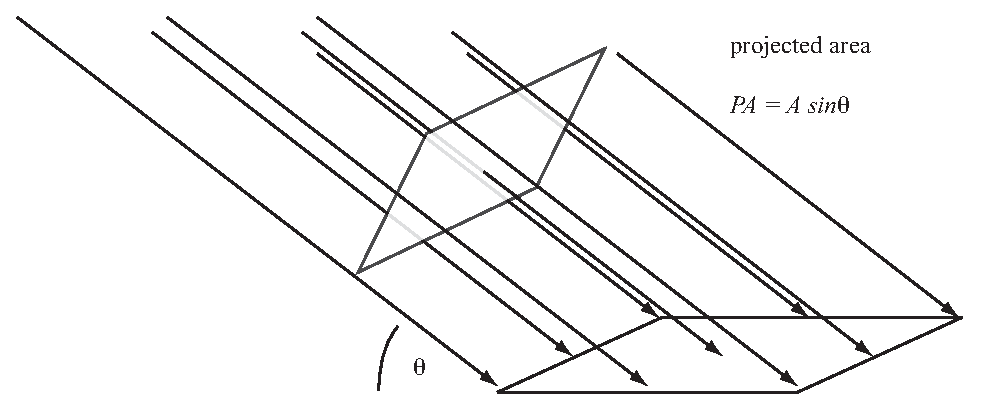
\includegraphics[height=1.5in]{figs/ProjectedArea}}
\afterfig

\subsection{Exercise: Freezing in Space}

In the cold, dark depths of space, the temperature is near to absolute zero.  Furthermore, the level of solar radiation can be quite high (e.g., at the distance of the earth from the sun, the solar insolation is 1366 $W/m^2$.  

Consequently,  at least according to wikipedia, one important requirement for space suits is  temperature regulation:

``Unlike on Earth, where heat can be transferred by convection to the atmosphere, in space heat can be lost only by thermal radiation or by conduction to objects in physical contact with the space suit. Since the temperature on the outside of the suit varies greatly between sunlight and shadow, the suit is heavily insulated, and the temperature inside the suit is regulated by a Liquid Cooling Garment in contact with the astronaut's skin, as well as air temperature maintained by the Primary Life Support System.''

Do you buy this?  How bad would it actually be if your space suit consisted of (say) a thin layer of shiny foil?  Would you freeze?  Would you burn up?  (set aside the pressure regulation question for now, although you might be interested in looking up Space Activity Suits to learn more about this...). 

\subsection{Convection}

The third way to transfer heat is by the actual motion of particles. Convection heat transfer occurs between a fluid in motion (usually a liquid or gas like water or air) and a bounding surface when the two are at different temperatures. You might imagine wearing shorts on a day with seasonal Arctic breezes (lots of heat transfer between your warm skin and the cold air). Convection can also occur in still air -- the fact that the air molecules can move around on their own (unlike the molecules in a solid which just vibrate in place) means that a still (or quiescent \sidenote{This is very fun word to say out loud. Go ahead, try it.}) gas or liquid can be spurred into motion in the presence of a temperature gradient. A hot surface (like a pan just pulled from the oven) heats the air around it, which causes the air to flow upwards, which brings cooler air into contact with the pan, effectively setting up a natural convection current around the pan. At a larger scale, most of the earth's weather is driven by convection processes.

Although it is easy to understand how convection leads to heat transport, there is not one uniform model for convective processes, as they often involve complex fluid dynamics.  Having said that, there are many situations in which you can build useful models for convective heat loss without getting into the weeds of fluid dynamics. The simplest model is called Newton's Law of Cooling (again, not a law, but a model):

$$ \dot Q=hA(T_\infty-T_s) $$

where $A$ is the area of the surface exposed to the convective currents, $T_\infty$ is the temperature of the surrounding fluid, $T_s$ is the temperature of the surface, and $h$ is known as the heat transfer coefficient, which is the key piece of information describing a given convective heat transfer physical system. The simplest approach to determining the heat transfer coefficient is to start with an estimate (using the table below) and then refine that estimate using empirical relationships found in any heat transfer text.

\begin{center}
Typical Values of the Convection Heat Transfer Coefficient 
\begin{tabular}{ | p{5cm} | p{2cm} | }
\hline
Process & $h (W/m^2 K) $\\
\hline
Natural convection -- Gases & 2 -- 25 \\
\hline
Natural convection -- Liquids & 50 -- 1000 \\
\hline
Forced convection -- Gases & 25 -- 250 \\
\hline
Forced convection -- Liquids & 50 -- 20,000 \\
\hline
\end{tabular}
\end{center}

\subsection{Volumetric Transfer}

Consider the case of going through a revolving door on a cold day.  When you do this, you exchange a volume $V$ of warm interior air for the same volume of cold, nasty exterior air.  Thus, this will lead to a change in internal energy of
$$ \Delta U = - V\rho c (T_{in} - T_{out})$$
where V is the exchanged volume of air, $\rho$ is the density of the air, and $c$ is the specific heat of the air.

Similarly, most houses lose air continually through poorly sealed windows, vents, etc.  If we assume that the rate of exchange is $\frac{dV}{dt}$ m$^3$/sec, the rate of change in the internal energy would be 
$$\frac{d\Delta U}{dt} = - \frac{dV}{dt} \rho c (T_{in} - T_{out})$$
This works as long as the flow is slow enough that the exiting air is at internal temperature.

\subsection{Boundary Layers}

Even when the actual mechanism of heat transfer is convection, it is often convenient, and accurate enough, to use a conductive model, by introducing an abstraction called a {\it boundary layer}. The basic idea here is that we imagine there is some thin layer of fluid near the interface that can be treated as if it were a thermal resistance.  

This is, in fact, not a crazy idea -- when an object is in a moving fluid, the velocity of the fluid at the surface of the object must be zero, and there is a thin distance (the boundary layer) over which the velocity rises to reach the free stream velocity.  This thin layer does tend to dominate the heat flow -- once heat gets to the free stream, it is quickly carried away.  Of course, convection {\it is} taking place within the boundary layer -- we are simply saying that the behavior of the boundary layer {\it looks like} conduction.  

Qualitatively, this model has explanatory power.  Think, for example, about a person going outside on a cold day.  The flow of heat out of the person will depend on the total thermal resistance that separates the person's core from the environment.  This total resistance will include:
\begin{itemize}
\item The thermal resistance of skin, fat, etc.: We abstract the person into a core (stock of internal energy) and a thermal resistance that connects that core to the surface of the body
\item The thermal resistance of air trapped between clothes and skin
\item The thermal resistance of cloth
\item The effective thermal resistance of the boundary layer
\end{itemize}
Qualitatively, this model says:
\begin{itemize}
\item Skinny people will get cold faster, because they have relatively low resistance between the core and the surface of the body
\item Goosedown coats will work well, because they increase the thickness of the trapped air layer
\item Heavy coats will work well, because they increase the resistance of the cloth
\item People will tend to get colder faster when it is windy, because the thickness of the boundary layer decreases with increasing wind speed.
\end{itemize}
Making this model quantitative requires some additional information / experimental results.  One option is to approximate the boundary layer thickness using a fluid dynamics approach (see wikipedia); another option would determine the thickness by comparing the time for heat to diffuse with the time for the fluid to travel over the object (see Sanjoy's book).  Either of these approaches will give you reasonable qualitative results; doing better will really require you to validate your heat transfer coefficient with some kind of empirical data.

